% ============================================================================
%   Comprehensive Research Report on the Universal MDEP Architecture
%   Mathematical Foundations, Multi-Agent Dynamics, and Clinical Applications
%
%   File: swin_mdep_report_en.tex
%   Version: 2.0 (Updated 06/2026)
%   Language: English
% ============================================================================

\documentclass[11pt, a4paper]{article}

% --- Packages ---
\usepackage[utf8]{inputenc}
\usepackage[english]{babel}
\usepackage{amsmath, amssymb, amsthm, bm}
\usepackage{graphicx}
\usepackage{booktabs}
\usepackage{float}
\usepackage{hyperref}
\usepackage{algorithm}
\usepackage{algorithmic}
\usepackage{enumitem}
\usepackage{geometry}
\usepackage{tikz}
\usetikzlibrary{arrows.meta, positioning}
\usepackage{xcolor}

\geometry{margin=2.5cm}

% --- Custom commands ---
\newcommand{\Dir}{\text{Dir}}
\newcommand{\KL}{\text{KL}}
\newcommand{\R}{\mathbb{R}}
\newcommand{\E}{\mathbb{E}}
\newcommand{\Norm}{\text{Norm}}
\newcommand{\softplus}{\text{Softplus}}

\newtheorem{remark}{Remark}
\newtheorem{proposition}{Proposition}

% ============================================================================
\title{
    \textbf{Universal MDEP Architecture} \\[6pt]
    \large Methodology, Mathematical Foundations, and Evidential Optimization
}
\author{Swin-MDEP Project}
\date{June 2026 --- Version 2.0}

\begin{document}
\maketitle

\section{Backbone Architectures: ResNet and Swin Transformer}\label{sec:backbones}

The Universal MDEP architecture is designed to be backbone-agnostic, enabling integration with both convolutional and transformer-based vision architectures. Understanding the structural properties of these backbones is essential to analyze how MDEP guides connection pruning and regrowth.

\subsection{ResNet: Deep Residual Learning}

In traditional deep neural networks, stacking more layers often leads to the degradation problem: beyond a certain depth, training accuracy saturates and then degrades rapidly. This is not caused by overfitting, but rather by optimization challenges like vanishing or exploding gradients. To overcome this, He et al.~\cite{he2016deep} introduced Deep Residual Learning, where layers are formulated to learn residual mappings with reference to the layer inputs. The basic residual block is defined as:
\begin{equation}\label{eq:residual_block}
    \mathbf{y} = \mathcal{F}(\mathbf{x}, \{W_i\}) + \mathbf{x}
\end{equation}
where $\mathbf{x}$ and $\mathbf{y}$ are the input and output vectors of the block, and the function $\mathcal{F}(\mathbf{x}, \{W_i\})$ represents the residual mapping to be learned. A skip connection (shortcut) performs identity mapping, which adds no parameters or computational complexity, permitting gradients to flow directly back to earlier layers. When a dimension change is required between the input and output (e.g., in downsampling blocks), a projection shortcut is used:
\begin{equation}\label{eq:residual_proj}
    \mathbf{y} = \mathcal{F}(\mathbf{x}, \{W_i\}) + W_s \mathbf{x}
\end{equation}
where $W_s$ is a linear projection layer.

The ResNet family employs two primary residual block designs:
\begin{enumerate}
    \item \textbf{BasicBlock}: Consists of two consecutive $3 \times 3$ convolutional layers. This is the fundamental block used in smaller ResNet variants such as ResNet-18 and ResNet-34.
    \item \textbf{Bottleneck Block}: Consists of a three-layer stack of $1 \times 1$, $3 \times 3$, and $1 \times 1$ convolutions. The initial $1 \times 1$ convolution reduces (bottlenecks) the channel dimension, the $3 \times 3$ convolution performs spatial processing, and the final $1 \times 1$ convolution restores the dimension. This design minimizes parameters and floating-point operations (FLOPs) in deeper variants like ResNet-50, ResNet-101, and ResNet-152.
\end{enumerate}

In the MDEP framework, the dense Evidential ResNet-18 teacher model utilizes a customized ResNet-18 backbone. Three reasons justify this specific selection over a heavier ResNet-50:
\begin{enumerate}[label=(\roman*)]
    \item \textbf{Overfitting Prevention:} The clinical ISIC 2024 dataset contains a extremely small number of rare positive cases (${\sim}390$). High-capacity models like ResNet-50 are prone to memorizing these samples, damaging their Dirichlet uncertainty estimation. The simpler ResNet-18 functions as an implicit regularizer.
    \item \textbf{Cross-Architecture Bias Distillation:} Distilling the strong local spatial inductive bias from the CNN teacher into the Swin Transformer student forces the student's Self-Attention mechanism to focus on lesion boundaries.
    \item \textbf{Hardware and Memory Constraints:} Distilling a student and teacher model simultaneously alongside the MDEP multi-agent system is highly memory-intensive; using ResNet-18 avoids out-of-memory errors on standard GPUs.
\end{enumerate}

\subsection{Vision Transformer (ViT) Fundamentals}

Unlike CNNs, which process images via local receptive fields, the Vision Transformer (ViT)~\cite{dosovitskiy2021image} applies the self-attention mechanism globally across the entire image. To process 2D images, ViT reshapes an image $\mathbf{X} \in \mathbb{R}^{H \times W \times C}$ into a sequence of flattened 2D patches $\mathbf{X}_p \in \mathbb{R}^{N \times (P^2 C)}$, where $P \times P$ is the patch size and $N = HW/P^2$ is the total number of patches. 

These patches are projected into a $D$-dimensional latent space via a trainable linear projection $\mathbf{E} \in \mathbb{R}^{(P^2 C) \times D}$ to yield patch embeddings. To retain spatial relationships, a learnable 1D positional encoding $\mathbf{E}_{\text{pos}} \in \mathbb{R}^{(N+1) \times D}$ is added to the patch embeddings along with a learnable classification token $\mathbf{x}_{\text{class}} \in \mathbb{R}^{1 \times D}$:
\begin{equation}\label{eq:vit_embedding}
    \mathbf{Z}_0 = [\mathbf{x}_{\text{class}}; \mathbf{X}_p \mathbf{E}] + \mathbf{E}_{\text{pos}}
\end{equation}
The sequence of tokens $\mathbf{Z}_0$ is then processed by a sequence of Transformer encoder blocks. Each block consists of a Multi-Head Self-Attention (MSA) and a Multi-Layer Perceptron (MLP) block, with Layer Normalization (LN) applied before each block and residual connections after. The core attention mechanism is:
\begin{equation}\label{eq:self_attention}
    \text{Attention}(Q, K, V) = \text{softmax}\left(\frac{QK^T}{\sqrt{d_k}}\right)V
\end{equation}
where queries $Q$, keys $K$, and values $V$ are projected from the input tokens.

\subsection{Swin Transformer Architecture}

Although ViT achieves excellent global context modeling, it suffers from two major limitations: the computational complexity of global self-attention is quadratic $\mathcal{O}(H^2 W^2)$ with respect to image resolution, and it produces single-scale features. The Swin (Shifted Window) Transformer~\cite{liu2021swin} resolves these limitations through a hierarchical architecture and local window attention.

\begin{enumerate}
    \item \textbf{Hierarchical Feature Maps:} Swin Transformer builds hierarchical feature representations by gradually merging patch layers in deeper stages (similar to the feature pyramids of CNNs). It outputs feature maps of resolutions $H/4 \times W/4$, $H/8 \times W/8$, $H/16 \times W/16$, and $H/32 \times W/32$, making it highly suitable for dense prediction and multi-scale feature alignment.
    
    \item \textbf{Local Window Self-Attention (W-MSA):} To reduce computational overhead, Swin Transformer partitions the feature map into non-overlapping local windows of size $M \times M$ (typically $M=7$) and computes self-attention exclusively within each window. This reduces the computational complexity from quadratic to linear:
    \begin{align}
        \text{Complexity of global self-attention (ViT):} \quad &\Omega(\text{Global}) = 4HWC^2 + 2(HW)^2 C \\
        \text{Complexity of window self-attention (W-MSA):} \quad &\Omega(\text{W-MSA}) = 4HWC^2 + 2HWM^2 C
    \end{align}
    Because $M^2$ is small and constant, the W-MSA complexity scales linearly with the image size $HW$.
    
    \item \textbf{Shifted Window Self-Attention (SW-MSA):} To introduce cross-window communication while preserving local attention efficiency, Swin Transformer uses a shifted window partitioning scheme. In consecutive layers, the window partition is shifted by $(\lfloor M/2 \rfloor, \lfloor M/2 \rfloor)$ pixels. Self-attention is then computed on the shifted window layout. To compute attention on shifted windows efficiently, a cyclic shift mechanism and attention masking are used, preventing the need to compute attention on padded regions and maintaining window-boundary isolation.
    
    \item \textbf{Patch Merging:} At the end of each stage, neighboring patches of size $2 \times 2$ are concatenated ($4C$ dimensions) and linearly projected to a $2C$-dimensional space. This downsamples the spatial resolution by $2\times$ and doubles the channel dimension.
\end{enumerate}

% ============================================================================
%  4. MATHEMATICAL FOUNDATIONS
% ============================================================================
\section{Mathematical Foundations: Subjective Logic and Dirichlet Distribution}\label{sec:math}

The MDEP system completely replaces the traditional softmax activation function at the classification layer and adopts mathematical foundations derived from Subjective Logic (SL)~\cite{josang2016subjective}. This theoretical framework formalizes the relationship between "evidence" gathered from data and the "belief" of the model, mapping the network's outputs directly to the concentration parameters of a Dirichlet distribution~\cite{sensoy2018evidential}. The Dirichlet distribution acts as a conjugate prior for the multinomial distribution, providing a deeper and more mathematically rigorous probabilistic interpretation.

\subsection{Dirichlet Distribution Parameterization and the Role of the Softplus Function}

For a $K$-class classification problem, instead of outputting probabilities, the MDEP network is designed to output a non-negative evidence vector $\bm{e} = [e_1, \ldots, e_K]^T \ge \bm{0}$ from raw logit outputs $\bm{z} \in \R^K$. To ensure that the evidence is non-negative, MDEP enforces the smooth Softplus activation function:
\begin{equation}\label{eq:softplus}
    e_c = \ln(1 + \exp(z_c)), \quad c = 1, \ldots, K
\end{equation}

\begin{remark}[Why not use ReLU?]
The Rectified Linear Unit (ReLU) function truncates all gradients for negative logits to exactly zero, trapping the evidence of that class permanently at $e_c = 0$, leading to a "frozen" Dirichlet system on the zero-evidence simplex.
\end{remark}

From the obtained evidence vector, the system constructs the Dirichlet concentration parameters $\bm{\alpha} = [\alpha_1, \ldots, \alpha_K]^T$ by adding a flat prior:
\begin{equation}\label{eq:alpha}
    \alpha_c = e_c + 1.0, \quad c = 1, \ldots, K
\end{equation}
The constant $1.0$ ensures that when the network predicts zero evidence ($\bm{e} = \bm{0}$), the distribution reverts to the flat prior $\Dir(\bm{1})$, representing the state of "complete prior ignorance". The total evidence of the system, also called the Dirichlet strength, is:
\begin{equation}\label{eq:S}
    S = \sum_{c=1}^K \alpha_c = \sum_{c=1}^K e_c + K
\end{equation}

On the $(K{-}1)$-dimensional probability simplex $\Delta^{K-1} = \{\bm{p} \in \R^K : p_c \ge 0, \sum_{c=1}^K p_c = 1\}$, the probability density function of the Dirichlet distribution $\Dir(\bm{\alpha})$ is expressed as:
\begin{equation}\label{eq:dirichlet_pdf}
    p(\bm{p} \mid \bm{\alpha}) = \frac{\Gamma\!\left(\sum_{c=1}^K \alpha_c\right)}{\prod_{c=1}^K \Gamma(\alpha_c)} \prod_{c=1}^K p_c^{\alpha_c - 1}
\end{equation}

The expected probability $\hat{p}_c$ of each class $c$, which is used to make the final classification decision, is the mean of the Dirichlet distribution:
\begin{equation}\label{eq:p_hat}
    \hat{p}_c = \E[p_c] = \frac{\alpha_c}{S}
\end{equation}
The variance of the predicted probability is $\text{Var}(p_c) = \frac{\alpha_c(S - \alpha_c)}{S^2(S + 1)}$, reflecting that as $S$ increases, the Dirichlet distribution becomes tighter, indicating high confidence. Conversely, as $S \to K$, the variance expands, indicating high uncertainty.

\subsection{Decomposition of Predictive Uncertainty: Epistemic and Aleatoric}\label{subsec:uncertainties}

The greatest advantage of using Subjective Logic and the Dirichlet distribution is the ability to mathematically decompose the predictive uncertainty into two orthogonal and distinct components.

\subsubsection{Epistemic Uncertainty (Model-Centric --- $u_e$)}

This uncertainty arises from the model's lack of knowledge, usually occurring when the model encounters out-of-distribution (OOD) data or minority samples that it has not learned well. In the language of Subjective Logic, it is defined as the vacant belief mass:
\begin{equation}\label{eq:u_e}
    u_e = \frac{K}{S} = \frac{K}{\sum_{c=1}^K \alpha_c}
\end{equation}

\begin{proposition}[Epistemic Uncertainty Bounds]
For any valid concentration vector $\bm{\alpha}$, the value of $u_e$ always lies in the interval $(0, 1]$. The maximum value $u_e = 1.0$ is achieved if and only if $\bm{e} = \bm{0}$, i.e., $S = K$. As $S \to \infty$, $u_e \to 0$.
\end{proposition}

$u_e$ acts as a compass, guiding the network architecture to identify representation areas that require more learning capacity.

\subsubsection{Aleatoric Uncertainty (Data-Centric --- $u_a$)}

Unlike $u_e$, aleatoric uncertainty cannot be reduced by collecting more data, as it measures statistical entropy, overlapping class boundaries, and measurement noise. It is defined using the digamma function $\psi(x) = \frac{d}{dx} \ln \Gamma(x)$ yielding the formulation~\cite{malinin2018predictive}:
\begin{equation}\label{eq:u_a}
    u_a = \sum_{c=1}^K \frac{\alpha_c}{S} \left[\psi(S + 1) - \psi(\alpha_c + 1)\right]
\end{equation}

\begin{proposition}[Non-negativity of $u_a$]
For any $K > 1$, since $\alpha_c < S$ and due to the strict monotonicity of the digamma function ($\psi'(x) > 0$ for all $x > 0$), we always have $\psi(S + 1) > \psi(\alpha_c + 1)$. This guarantees that every term in the summation is positive, mathematically ensuring $u_a \ge 0$. In practical implementations, to protect against floating-point inaccuracies, $u_a \leftarrow \max(u_a, 0.0)$ should be applied.
\end{proposition}

% ============================================================================
%  5. DYNAMIC SPARSE TRAINING DYNAMICS
% ============================================================================
\section{Dynamic Sparse Training Dynamics and Smoothing Estimators}\label{sec:sparse}

\begin{figure}[htbp]
\centering
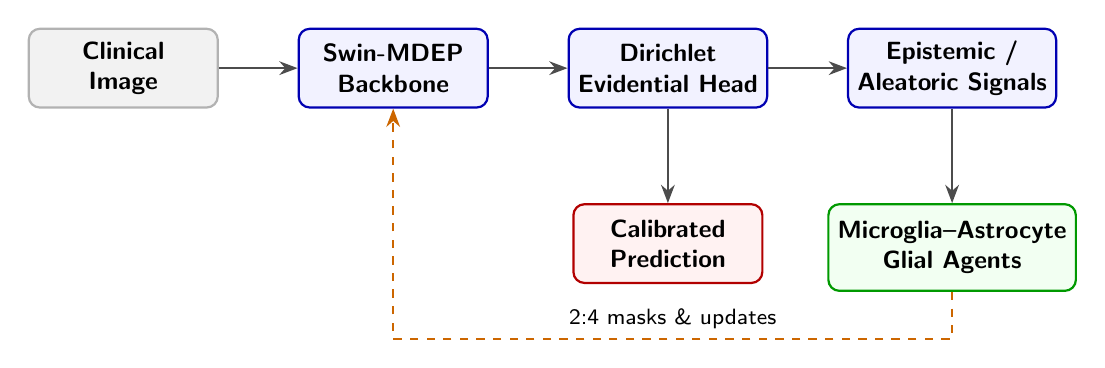
\begin{tikzpicture}[
    node distance=1.2cm and 1.0cm,
    box/.style={
        draw=blue!70!black,
        fill=blue!5,
        rounded corners,
        align=center,
        minimum width=2.4cm,
        minimum height=1cm,
        font=\small\sffamily\bfseries,
        thick
    },
    agent/.style={
        draw=green!60!black,
        fill=green!5,
        rounded corners,
        align=center,
        minimum width=2.6cm,
        minimum height=1.1cm,
        font=\small\sffamily\bfseries,
        thick
    },
    pred/.style={
        draw=red!70!black,
        fill=red!5,
        rounded corners,
        align=center,
        minimum width=2.4cm,
        minimum height=1cm,
        font=\small\sffamily\bfseries,
        thick
    },
    arrow/.style={
        ->,
        >=Stealth,
        thick,
        draw=black!70
    },
    feedback/.style={
        ->,
        >=Stealth,
        thick,
        dashed,
        draw=orange!80!black
    }
]

% Nodes
\node (img) [box, fill=gray!10, draw=gray!60] {Clinical\\Image};
\node (backbone) [box, right=of img] {Swin-MDEP\\Backbone};
\node (head) [box, right=of backbone] {Dirichlet\\Evidential Head};
\node (signals) [box, right=of head] {Epistemic /\\Aleatoric Signals};
\node (agents) [agent, below=of signals] {Microglia--Astrocyte\\Glial Agents};
\node (pred) [pred, below=of head] {Calibrated\\Prediction};

% Paths
\draw [arrow] (img) -- (backbone);
\draw [arrow] (backbone) -- (head);
\draw [arrow] (head) -- (signals);
\draw [arrow] (head) -- (pred);
\draw [arrow] (signals) -- (agents);
\draw [feedback] (agents.south) -- ++(0,-0.6) -| node[above, pos=0.25, font=\footnotesize\sffamily] {2:4 masks \& updates} (backbone.south);

\end{tikzpicture}
\caption{Overview of the Universal MDEP architecture instantiated as Swin-MDEP with a Swin Transformer backbone. Evidential uncertainty is used both for calibrated prediction and for dynamic sparse topology adaptation.}
\label{fig:overview}
\end{figure}

The philosophical starting point of the MDEP architecture is the separation of representation weight learning and network morphology learning into two parallel and independent dynamical systems. MDEP breaks with tradition by treating each layer as a system governed by two tiers of variables.

\subsection{Prediction Tier and Latent Morphological Tier}\label{subsec:two_tiers}

\paragraph{Prediction tier.}
Consists of the real weights $\bm{W}^{(l)}$, representing the traditional connection strengths of the network. These weights are responsible for minimizing the loss function and are continuously updated by standard optimizers such as AdamW.

\paragraph{Morphological tier.}
Contains a tensor of continuous latent scores $\bm{S}^{(l)}$ representing the potential "vitality" of each connection. For linear projection layers, $\bm{S}^{(l)} \in \R^{d_{\text{out}} \times d_{\text{in}}}$, while for convolutional layers, $\bm{S}^{(l)} \in \R^{C_{\text{out}} \times C_{\text{in}} \times K_h \times K_w}$. The binary mask matrix $\bm{M}^{(l)}$ is derived directly from $\bm{S}^{(l)}$ and determines which weights are allowed to survive to participate in the forward pass.

\begin{remark}[Isolating $\bm{S}$ from the Optimizer]
The structural scores $\bm{S}^{(l)}$ must be completely isolated from the parameters managed by the AdamW optimizer. If $\bm{S}$ is passed to AdamW, weight decay will gradually compress the structural memory to $\bm{0}$, causing "optimizer hijacking" and destroying the intended impulses generated by the biological agents. $\bm{S}$ is only allowed to update based on the internal dynamics of MDEP.
\end{remark}

\paragraph{Score initialization.}
At initialization, the latent scores are set to the absolute magnitude of the pre-trained weights:
\begin{equation}\label{eq:score_init}
    S_{ij}^{(0)} = |W_{ij}^{(l)}|
\end{equation}
If random initialization is used, the binary mask will blindly disable 50\% of the features, destroying the pre-trained knowledge base and causing a "Pruning Shock" from which model performance cannot recover.

\subsection{Enforcing NVIDIA 2:4 Structured Sparsity}\label{subsec:nvidia24}

Unstructured pruning methods do not deliver practical hardware acceleration benefits~\cite{hoefler2021sparsity}. To resolve this, MDEP enforces the NVIDIA 2:4 structured sparsity constraint~\cite{mishra2021accelerating, nvidia2020a100}: for every group of four consecutive elements along the input dimension, at most two elements are allowed to be non-zero~\cite{zhou2021learning, hubara2021accelerated}. 

Specifically, for a linear layer, each block $b$ represents 4 consecutive elements along the input dimension $d_{\text{in}}$. For a convolutional layer, the 2:4 structured sparsity is enforced along the input channel dimension $C_{\text{in}}$, meaning for each output channel $i$ and spatial coordinate $(y, x)$, every block of 4 elements along the input channel dimension contains at most 2 active connections.

\paragraph{Local survival threshold.}
The score matrix $\bm{S}$ is divided into blocks $\mathcal{B}$, each containing 4 elements. Within a block $b$, the four scores are sorted in descending order: $s_{1,b}^{(t)} \ge s_{2,b}^{(t)} \ge s_{3,b}^{(t)} \ge s_{4,b}^{(t)}$. The local survival threshold is:
\begin{equation}\label{eq:tau}
    \tau_b^{(t)} = \frac{1}{2} \left(s_{2,b}^{(t)} + s_{3,b}^{(t)}\right)
\end{equation}

\paragraph{Discrete binary mask.}
The mask $\bm{M}$ is determined via the Top-2-of-4 operator:
\begin{equation}\label{eq:mask}
    M_{i, 4k+j} = \begin{cases}
        1.0 & \text{if } S_{i, 4k+j} \ge \tau_{i,k} \\
        0.0 & \text{otherwise}
    \end{cases}
\end{equation}
The effective weights used in activation layers are $\bm{W}_{\text{eff}} = \bm{W} \odot \bm{M}$. This constraint guarantees exactly 50\% sparsity at the micro-level, yielding up to a 2$\times$ throughput speedup on Ampere and Hopper Tensor Cores.

\subsection{Localized Smoothed Straight-Through Estimator (Smoothed STE)}\label{subsec:ste}

Since the Top-2 operator generates a discrete binary mask, its derivative does not exist at almost any point~\cite{bengio2013estimating}. To resolve this propagation barrier, MDEP utilizes a Localized Smoothed Straight-Through Estimator.

\paragraph{Forward Pass:} The network uses the hard binary mask $\bm{M}$ to ensure actual 2:4 structured sparsity.

\paragraph{Backward Pass:} The gradient of the step function is approximated using the derivative of a sigmoid function centered at the local survival threshold:
\begin{equation}\label{eq:ste_grad}
    \frac{\partial M_{ij}}{\partial S_{ij}} \approx \frac{1}{\gamma_t} \sigma\!\left(\frac{S_{ij} - \tau_b^{(t)}}{\gamma_t}\right) \left[1 - \sigma\!\left(\frac{S_{ij} - \tau_b^{(t)}}{\gamma_t}\right)\right]
\end{equation}
where $\sigma(x) = (1 + \exp(-x))^{-1}$ is the sigmoid function, and $\gamma_t$ is the temperature parameter. Key characteristic: the derivative only peaks at $S_{ij} = \tau_b^{(t)}$, so structural gradients only flow strongly into scores that are currently competing at the live/die boundary within the same 2:4 block.

\paragraph{Temperature schedule.}
The temperature $\gamma(t)$ is decayed via a cosine schedule:
\begin{equation}\label{eq:gamma_schedule}
    \gamma(t) = \gamma_{\text{final}} + \frac{\gamma_{\text{initial}} - \gamma_{\text{final}}}{2}\left[1 + \cos\!\left(\pi \cdot \frac{t - t_w}{T - t_w}\right)\right]
\end{equation}
with $\gamma_{\text{initial}} = 5.0$ and $\gamma_{\text{final}} = 0.15$. Keeping the floor at $0.15$ instead of decaying to $0$ ensures that boundary gradients do not completely vanish as the network converges.

\begin{remark}[STE Dynamics and Connection Freezing Prevention]
We highlight that the continuous latent scores $S_{ij}$ are not directly updated using backpropagated gradients flowing through the STE. Instead, they are updated directly by the glial agents via the EMA of the score updates $\Delta S_{ij} = G_{ij} - C_{ij}$. Therefore, the fact that the sigmoid derivative in Equation~\ref{eq:ste_grad} approaches zero away from the threshold $\tau_b^{(t)}$ does not freeze the regrowth of pruned connections. Exploration and regrowth of pruned connections (where the weight gradient is indeed 0) is driven by the stochastic anti-crystallization noise term $\epsilon_{ij}$ (Equation~\ref{eq:anti_crystal_eq}) scaled by the node's epistemic uncertainty.
\end{remark}

\paragraph{Morphological Cache Optimization.}
In the naive implementation, the discrete mask $\bm{M}$ and local survival thresholds $\bm{\tau}$ are recomputed via sorting (\texttt{torch.sort}) and search (\texttt{torch.topk}) operations over all weights in \emph{every forward pass of every mini-batch}. Since the latent scores $\bm{S}$ are updated only once at the beginning of each epoch (at batch 0), performing these sorting operations on tens of millions of parameters at every mini-batch step is redundant and introduces a severe performance bottleneck.

To resolve this design flaw, Swin-MDEP introduces the Morphological Cache mechanism. The threshold $\bm{\tau}$ is registered as a non-persistent buffer (\texttt{persistent=False}) inside the \texttt{MDEPLinear} and \texttt{MDEPConv2d} layers. Both the binary mask $\bm{M}$ and thresholds $\bm{\tau}$ are calculated once at the end of the warmup phase or when updating the network structure at the start of each epoch; they are then stored and reused directly across all remaining mini-batches of that epoch. Setting \texttt{persistent=False} avoids checkpoint pollution, maintaining backward compatibility with pre-trained weights. This optimization removes redundant sorting operations, lowers CPU/GPU resource overhead, and significantly accelerates the forward pass.

% ============================================================================
%  6. BIOLOGICALLY-INSPIRED INTERACTIVE DYNAMICS
% ============================================================================
\section{Biologically-Inspired Interactive Dynamics: Microglia and Astrocyte Multi-Agent System}\label{sec:agents}

The soul of the MDEP architecture lies in its dynamic connection topology updates, driven by two agents inspired by the brain's glial system~\cite{paolicelli2011synaptic, schafer2012microglia}. We note that in biological neurodevelopment, the interaction between glial cells and synapses is highly complex; for example, astrocytes not only promote synaptogenesis but also participate in synaptic pruning through MEGF10 and MERTK pathways~\cite{chung2013astrocytes}, and microglia engage in detailed crosstalk with astrocytes~\cite{vainchtein2018astrocyte}. Within the MDEP framework, we adopt a simplified computational abstraction where the Microglia and Astrocyte agents are assigned distinct, orthogonal roles (pruning and growing, respectively) to enable decoupled control over network connection density and explore the topological search space efficiently. While standard compression algorithms simply prune weights with the smallest absolute values~\cite{han2016deep}, MDEP redistributes the computation graph by balancing task representation requirements against the spread of uncertainty.

\subsection{Microglia Agent: Pruning Noisy Evidence}\label{subsec:microglia}

In the human brain, microglia are responsible for clearing redundant or damaged synapses~\cite{paolicelli2011synaptic, schafer2012microglia}. In MDEP, this agent eliminates connections that amplify "garbage evidence" stemming from data noise. The agent evaluates each link based on two sensitivity spectra via first-order Taylor expansion:

\paragraph{Task-predictive sensitivity ($c_1$):}
Reflects how much a connection $w_{ij}$ contributes to optimizing the task loss function:
\begin{equation}
    c_1^{(ij)} = \left| w_{ij} \cdot \frac{\partial L_{\text{EFL}}}{\partial w_{ij}} \right|
\end{equation}

\paragraph{Noisy sensitivity ($c_2$):}
Reflects the degree to which a connection absorbs or is affected by aleatoric uncertainty:
\begin{equation}
    c_2^{(ij)} = \left| w_{ij} \cdot \frac{\partial u_a}{\partial w_{ij}} \right|
\end{equation}

After local min-max normalization per layer to the interval $[0, 1]$, the composite pruning prevention score is defined as:
\begin{equation}\label{eq:C_ij}
    C_{ij} = \text{Norm}(c_1^{(ij)}) + \beta \cdot \text{Norm}(c_2^{(ij)})
\end{equation}
Connections with the lowest $C_{ij}$ are deemed useless and targeted for latent score suppression.

\begin{remark}[Mathematical Stability of Microglia Gradients]
The gradient of the aleatoric uncertainty $u_a$ with respect to the weight requires evaluating the trigamma function $\psi_1(x)$. Because MDEP enforces a prior offset of $+1.0$ (such that $\alpha_c = e_c + 1.0 \ge 1.0$), the arguments to the trigamma function in the derivative of $u_a$ are strictly bounded by $\alpha_c + 1 \ge 2.0$ and $S + 1 \ge K + 1 \ge 3.0$. Since the trigamma function $\psi_1(x)$ is monotonically decreasing for $x > 0$, we have $\psi_1(\alpha_c+1) \le \psi_1(2) \approx 0.645$ and $\psi_1(S+1) \le \psi_1(3) \approx 0.395$. This flat Dirichlet prior offset guarantees that the trigamma terms never explode, ensuring stable Microglia gradients.
\end{remark}

\subsection{Astrocyte Agent: Locating and Promoting Evidence Growth}\label{subsec:astrocyte}

Opposing the destructive force of the Microglia, the Astrocyte agent promotes weight growth in areas of the network experiencing representation deficiency~\cite{chung2013astrocytes, vainchtein2018astrocyte}. The Astrocyte targets neurons exhibiting high epistemic uncertainty ($u_e$).

\paragraph{Node-level feedback.}
$u_{e,i}^{(\text{node})}$ is computed via forward hooks. The potential growth signal is:
\begin{equation}\label{eq:G_ij}
    G_{ij} = \text{Norm}\!\left(\text{Expand}(u_e^{(\text{node})})\right) \cdot \text{Norm}\!\left(\left|\frac{\partial L_{\text{EFL}}}{\partial w_{ij}}\right|\right)
\end{equation}
This multiplicative formulation acts as a strict filter: a connection is only regrown if it connects to a node with high epistemic uncertainty \emph{and} has a strong task learning gradient.

\begin{remark}[Spatial Sensitivity of Astrocyte]
Although the class-wise derivative $\partial u_e / \partial \alpha_c = -K/S^2$ is a global scalar, the gradient backpropagated to an internal activation node $a_i^{(l)}$ is computed as $\frac{\partial u_e}{\partial a_i^{(l)}} = -\frac{K}{S^2} \sum_c \frac{\partial \alpha_c}{\partial a_i^{(l)}}$. The summation term represents the sensitivity of the total evidence $S$ to changes in $a_i^{(l)}$, which varies non-uniformly across channels and spatial coordinates depending on the network's weights and activations. Thus, the Astrocyte agent is not spatially blind and selectively targets connections with the greatest influence on total evidence.
\end{remark}

\subsection{Anti-Crystallization}\label{subsec:anti_crystal}

If an entire layer lacks any candidate connections offering useful growth gradients ($\max_{ij} G_{ij} \le 10^{-8}$), MDEP injects an emergency response:
\begin{equation}\label{eq:anti_crystal_eq}
    \tilde{G}_{ij} = G_{ij} + \max\!\left(0.0,\; \epsilon_{ij} \cdot \text{Norm}(u_{e,i}^{(\text{node})})\right)
\end{equation}
where $\epsilon_{ij} \sim \mathcal{N}(0, 0.0316^2)$. Due to the multiplicative structure, the system prioritizes "experimenting" by opening new links in regions lacking evidence.

\subsection{Latent Score Updates via EMA}\label{subsec:score_update}

Continuous score updates are calculated at the end of each training step by combining the opposing forces of growth and pruning:
\begin{equation}\label{eq:delta_S}
    \Delta S_{ij} = G_{ij} - C_{ij}
\end{equation}
To smooth gradient fluctuations across mini-batches, score momentum is applied:
\begin{align}
    V_{ij}^{(t)} &= \beta_m V_{ij}^{(t-1)} + (1 - \beta_m) \Delta S_{ij} \\
    S_{ij}^{(t)} &= S_{ij}^{(t-1)} + \eta V_{ij}^{(t)}
\end{align}
where $\beta_m = 0.95$ is the EMA coefficient, and $\eta = 0.02$ is the structural update rate. To prevent score saturation (which would permanently lock connections), MDEP centers and clamps the scores:
\begin{align}
    S_{ij}^{(t)} &\leftarrow S_{ij}^{(t)} - \text{mean}(\bm{S}^{(t)}) \\
    S_{ij}^{(t)} &\leftarrow \text{clamp}(S_{ij}^{(t)}, -5.0, 5.0)
\end{align}
This centering ensures that the average latent score of each layer remains 0, maintaining healthy competition among links.

\begin{remark}[Role of Residual Connections]
The residual connections in both ResNet-50 and Swin Transformer act as safe bypass routes. By preserving identity mapping pathways, they protect spatial information flow from abrupt topological disruption when the network applies 50\% parameter structured sparsity.
\end{remark}

\subsection{Integration with ResNet-50 (ResNet-MDEP)}\label{subsec:resnet}

Applying MDEP's bi-directional sparsity updates to the convolutional ResNet-50 backbone requires wrapping its internal layers. Inside each residual Bottleneck block of ResNet-50, we replace all convolutional layers with our sparse \texttt{MDEPConv2d} layers, including:
\begin{itemize}
    \item \texttt{conv1}: $1 \times 1$ convolution for bottleneck channel reduction.
    \item \texttt{conv2}: $3 \times 3$ convolution for spatial feature processing.
    \item \texttt{conv3}: $1 \times 1$ convolution for bottleneck channel expansion.
\end{itemize}

\paragraph{Preserving Low-Level Features.}
Just as with the patch projection in transformers, the first convolution of the ResNet-50 network (\texttt{conv1}, a $7 \times 7$ conv with stride 2 and padding 3) operates directly on the raw input pixels and is parameter-light. Enforcing structured sparsity at this entry point would filter out crucial visual details. Consequently, the initial convolutional layer is explicitly excluded from MDEP and remains dense.

\paragraph{Convolutional Activation Gradient Pooling.}
For convolutional layers, the activation gradient is a 4D tensor. Let $\bm{g}_{\text{act}}^{(l)} = \frac{\partial \bar{u}_e}{\partial \bm{a}^{(l)}} \in \R^{B \times C_{\text{out}} \times H \times W}$ represent the gradient of mean epistemic uncertainty with respect to the layer's output activation tensor. To define a node-level uncertainty signal for each channel, the Astrocyte agent pools this gradient over batch and spatial dimensions:
\begin{equation}\label{eq:conv_pooling}
    u_{e,i}^{(\text{node})} = \frac{1}{B \cdot H \cdot W} \sum_{b=1}^B \sum_{y=1}^H \sum_{x=1}^W \left| g_{\text{act}, i}^{(l)}(b, y, x) \right|
\end{equation}
yielding a channel-wise vector $\bm{u}_e^{(\text{node})} \in \R^{C_{\text{out}}}$. This vector is then expanded to match the dimensions of the convolutional weights $\bm{W}^{(l)} \in \R^{C_{\text{out}} \times C_{\text{in}} \times K_h \times K_w}$:
\begin{equation}
    g_{1, ijkx} = u_{e,i}^{(\text{node})}
\end{equation}
which ensures the Astrocyte growth signal is aligned with weight-level gradients.

\subsection{Compatibility with Swin Transformer (Swin-MDEP)}\label{subsec:swin}

Adapting MDEP to the Swin Transformer~\cite{liu2021swin, liu2022swinv2} introduces more complex challenges. In the 4-stage hierarchical Swin-MDEP, all linear projections inside the self-attention and MLP blocks are replaced with sparse \texttt{MDEPLinear} layers, including:
\begin{itemize}
    \item \texttt{attn.qkv}: Query, Key, Value projection layer.
    \item \texttt{attn.proj}: Linear output attention projection.
    \item \texttt{mlp.fc1} and \texttt{mlp.fc2}: Hidden channel expansion and contraction layers.
\end{itemize}

\paragraph{Preserving the Patch Partition.}
The initial patch projection layer (\texttt{Conv2D(3, 96, kernel\_size=4, stride=4)}) has a tiny parameter count (only 4,608 weights) but is responsible for extracting raw RGB features. Enforcing 2:4 structured sparsity here would force the network to discard 50\% of the raw pixel information at the gateway of the system. Therefore, this layer is explicitly excluded from MDEP sparsification.

\paragraph{Generalized Activation Gradient Pooling Operator.}
Since activation tensors vary in shape across Swin's stages due to Patch Merging, Swin-MDEP introduces a generalized pooling operator. Let $\bm{g}_{\text{act}}^{(l)} = \frac{\partial \bar{u}_e}{\partial \bm{a}^{(l)}}$ be the gradient of the mean epistemic uncertainty $\bar{u}_e = \frac{1}{N}\sum_n u_{e,n}$ with respect to the layer activation $\bm{a}^{(l)}$. By averaging the absolute value of this gradient over all spatial dimensions (excluding the channel dimension), the high-dimensional tensor is reduced to a 1D vector $\bm{u}_e^{(\text{node})} \in \R^D$:
\begin{equation}\label{eq:activation_pooling}
    \bm{u}_e^{(\text{node})} = \text{mean}\!\left(|\bm{g}_{\text{act}}^{(l)}|,\; \text{dim}=[0, 1, \ldots, \text{ndim}-2]\right)
\end{equation}
This establishes a uniform basis for the Astrocyte agent, permitting evaluation of channel-wise evidence hunger regardless of spatial resolution.

% ============================================================================
%  7. OPTIMIZATION FRAMEWORK
% ============================================================================
\section{Optimization Framework: Evidential Focal Loss and Distillation Protocol}\label{sec:optimization}

\subsection{Evidential Focal Loss (EFL)}\label{subsec:efl}

When facing extreme class imbalance---such as in the ISIC 2024 cohort~\cite{isic2024} where malignant cases account for only $0.15\%$~\cite{johnson2019survey}---standard loss functions collapse. While the term Evidential Focal Loss has been used in prior literature (e.g., Zhou et al.~\cite{zhou2023domain} for prostate cancer classification), our Evidential Focal Loss (EFL) formulation is customized to combine digamma-based cross-entropy (introduced by Sensoy et al.~\cite{sensoy2018evidential}) with a dynamic focal modulation term (Lin et al.~\cite{lin2017focal}) and frequency-dampened class weights, specifically structured for active sparsity in highly imbalanced skin lesion screening. EFL is designed to be formulated as follows:
\begin{equation}\label{eq:efl}
    L_{\text{EFL}}(\bm{e}, \bm{y}, t) = \frac{1}{N} \sum_{n=1}^N \omega_n \left[\mathcal{F}(t) \cdot L_{\text{CE}}^{(n)} + \lambda_{\text{KL}} \cdot \mu(t) \cdot L_{\text{KL}}^{(n)}\right]
\end{equation}
where $N$ is the mini-batch size, $\bm{y}^{(n)} \in \{0, 1\}^K$ is the one-hot target of sample $n$, and $\omega_n = \sum_{c=1}^K y_c^{(n)} \omega_c$ is the class-balanced sample weight.

\paragraph{Digamma-Based Cross-Entropy ($L_{\text{CE}}$):}
\begin{equation}
    L_{\text{CE}}^{(n)} = \sum_{c=1}^K y_c^{(n)} \left[\psi(S^{(n)}) - \psi(\alpha_c^{(n)})\right]
\end{equation}

\paragraph{Dynamic Focal Modulation ($\mathcal{F}(t)$):}
\begin{equation}
    \mathcal{F}(t) = \left(1 - \text{sg}[\hat{p}_{\text{target}}^{(n)}]\right)^{\gamma(t)}
\end{equation}
where $\hat{p}_{\text{target}}^{(n)} = \sum_{c=1}^K y_c^{(n)} \hat{p}_c^{(n)}$ is the expected probability of the true class, and $\text{sg}[\cdot]$ is the stop-gradient operator (implemented via \texttt{.detach()} in PyTorch) to prevent backpropagation through the focal weight, which would otherwise distort the Dirichlet distribution. During the warmup phase, $\gamma(t) = 0$ to establish a stable baseline. In later phases, $\gamma$ is gradually scaled up to $1.2$ to focus on hard samples.

\paragraph{Dampened Class Weights ($\omega_c$):}
\begin{equation}\label{eq:class_weights}
    \omega_c = \sqrt{N_{\text{total}} / N_c}
\end{equation}
Following Cui et al.~\cite{cui2019class}, this square-root scaling dampens the actual imbalance ratio of $670{:}1$ to a weight of approximately $25.9$ for the malignant class (melanoma)---strong enough to provide gradient force, yet safe enough to maintain numerical stability.

\paragraph{Independent KL Regularization ($L_{\text{KL}}$):}
This term suppresses spurious evidence. By modifying the concentration vector $\tilde{\bm{\alpha}}^{(n)}$, it preserves the evidence of the correct class while shrinking the concentrations of incorrect classes to the flat prior $1.0$:
\begin{equation}
    \tilde{\alpha}_c^{(n)} = y_c^{(n)} + (1 - y_c^{(n)}) \cdot \alpha_c^{(n)}
\end{equation}
The regularizer is computed as the analytical KL divergence between the adjusted Dirichlet distribution and the flat prior $\Dir(\bm{1})$:
\begin{align}
    L_{\text{KL}}^{(n)} &= \KL\!\left(\Dir(\tilde{\bm{\alpha}}^{(n)}) \,\|\, \Dir(\bm{1})\right) \nonumber \\
    &= \ln \left( \frac{\Gamma\left(\sum_{c=1}^K \tilde{\alpha}_c^{(n)}\right)}{\Gamma(K) \prod_{c=1}^K \Gamma(\tilde{\alpha}_c^{(n)})} \right) + \sum_{c=1}^K (\tilde{\alpha}_c^{(n)} - 1)\left[\psi(\tilde{\alpha}_c^{(n)}) - \psi\!\left(\sum_{c=1}^K \tilde{\alpha}_c^{(n)}\right)\right] \label{eq:kl_loss_n}
\end{align}
where $\psi(\cdot)$ is the digamma function, and the scaling coefficient is $\mu(t) = \min(1.0, t / t_{\text{anneal}})$ with $t_{\text{anneal}} = 10$, allowing the network to explore representations before enforcing strict evidence penalties.

\begin{remark}[Independence of $L_{\text{KL}}$ and Focal Coefficient]
The KL divergence term is not multiplied by $\mathcal{F}(t)$. If it were, the model would lower the penalty for easy majority samples, allowing spurious evidence to accumulate unchecked.
\end{remark}

\subsection{Dirichlet KL Knowledge Distillation}\label{subsec:distillation}

To stabilize the sparse Swin-T student network during its transition to 2:4 structured sparsity, the system applies knowledge distillation techniques~\cite{hinton2015distilling, gou2021knowledge}, specifically evidential distribution distillation~\cite{malinin2019ensemble} from a fully converged dense Evidential ResNet-18 teacher model~\cite{he2016deep}.

\begin{remark}[Why ResNet-18 instead of ResNet-50 as Teacher?]
Three main reasons justify this selection:
\begin{enumerate}[label=(\roman*)]
    \item \textbf{Cross-Architecture Inductive Bias:} ResNet-18 is a pure CNN with strong local spatial inductive biases. Distilling from a CNN to a ViT helps transfer spatial locality to Swin-T's Self-Attention mechanism, focusing attention on lesion regions.
    \item \textbf{Preventing Overfitting on Rare Minority Classes:} A ResNet-50 teacher is highly complex (50 layers with bottleneck blocks) and prone to memorizing the small number of malignant samples (${\sim}390$), which distorts its Dirichlet uncertainty estimation ($\bm{\alpha}_T$). ResNet-18 is simpler and acts as a regularizer, providing better-calibrated teacher distributions.
    \item \textbf{VRAM Optimization:} Hosting both the teacher and student networks in GPU memory alongside the MDEP engine during training is memory-intensive. ResNet-18 (${\sim}11.7$M parameters) avoids Out-of-Memory (OOM) errors on standard GPUs (e.g., T4 with 15--16GB VRAM), whereas ResNet-50 (${\sim}25.6$M parameters) easily triggers VRAM overflow.
\end{enumerate}
\end{remark}

\paragraph{Teacher Model Configuration.}
The teacher is a customized dense Evidential ResNet-18 with an evidential classification head ($\text{Linear}(512, K) \to \softplus(\cdot)$) and dense \texttt{MDEPConv2d}/\texttt{MDEPLinear} layers (with MDEP pruning disabled), pre-trained to convergence on the ISIC 2024 dataset.

\paragraph{Dynamic Path Resolution.}
To ensure seamless execution across local development environments and cloud platforms (such as Kaggle), the system automatically scans candidate paths for the teacher checkpoint (\texttt{model\_checkpoint.pth}):
\begin{enumerate}
    \item Current working directory: \texttt{model\_checkpoint.pth}
    \item Parallel directory: \texttt{../RESNET50 backbone/model\_checkpoint.pth}
    \item Local subdirectory: \texttt{./RESNET50 backbone/model\_checkpoint.pth}
    \item Kaggle input path: \texttt{/kaggle/input/mdep-resnet50-backbone/model\_checkpoint.pth}
\end{enumerate}
The teacher weights are loaded from the first matching path, and the teacher model is frozen (\texttt{requires\_grad = False}).

\paragraph{Distillation Loss Formulation.}
The analytical KL divergence between the student and teacher Dirichlet distributions is formulated as:
\begin{align}
    \KL(\Dir(\bm{\alpha}_S) \| \Dir(\bm{\alpha}_T)) &= \ln\Gamma(S_S) - \ln\Gamma(S_T) - \sum_{c=1}^K \left[\ln\Gamma(\alpha_{S,c}) - \ln\Gamma(\alpha_{T,c})\right] \nonumber \\
    &\quad + \sum_{c=1}^K (\alpha_{S,c} - \alpha_{T,c})\left[\psi(\alpha_{S,c}) - \psi(S_S)\right] \label{eq:dir_kl_full}
\end{align}
The distillation weight $\alpha_d(t)$ is scheduled via a cosine decay function:
\begin{equation}\label{eq:alpha_d}
    \alpha_d(t) = \begin{cases}
        \alpha_{d,\text{init}} & \text{if } t < t_w \\[6pt]
        \alpha_{d,\text{final}} + \dfrac{\alpha_{d,\text{init}} - \alpha_{d,\text{final}}}{2}\left[1 + \cos\!\left(\pi \cdot \dfrac{t - t_w}{T - t_w}\right)\right] & \text{if } t \ge t_w
    \end{cases}
\end{equation}
with $\alpha_{d,\text{init}} = 0.5$ and $\alpha_{d,\text{final}} = 0.05$. The total loss is:
\begin{equation}\label{eq:total_loss}
    L_{\text{total}} = L_{\text{EFL}}(\bm{e}_S, \bm{y}, t) + \alpha_d(t) \cdot L_{\text{distill}}
\end{equation}

Crucially, while Swin-MDEP relies on this distillation protocol, the convolutional ResNet-50 MDEP model is trained in a self-contained manner directly using the Evidential Focal Loss (Equation~\ref{eq:efl}) without a teacher model.

\paragraph{Three-Fold Role of Knowledge Distillation:}
\begin{enumerate}
    \item \textbf{Sensitivity Improvement:} The teacher provides "soft" evidential distributions, assisting the student in separating ambiguous boundaries.
    \item \textbf{Better Uncertainty Calibration:} The distillation loss aligns the student's Dirichlet parameters with the teacher's, reducing the student's ECE.
    \item \textbf{Sparsity Protection:} The KD loss provides a regularization force that guides weight optimization when 50\% of the connections are pruned.
\end{enumerate}

% ============================================================================
%  8. EXPERIMENTAL SETUP
% ============================================================================

\begin{thebibliography}{99}

\bibitem{bengio2013estimating}
Y.~Bengio, N.~L{\'e}onard, and A.~Courville.
\newblock Estimating or propagating gradients through stochastic neurons for conditional computation.
\newblock {\em arXiv preprint arXiv:1308.3432}, 2013.

% ===== KNOWLEDGE DISTILLATION =====

\bibitem{chung2013astrocytes}
W.S.~Chung, L.E.~Clarke, G.X.~Wang, B.K.~Stafford, A.~Sher, C.~Chakraborty, J.~Joung, L.C.~Foo, A.~Thompson, C.~Chen, S.J.~Smith, and B.A.~Barres.
\newblock Astrocytes mediate synapse elimination through MEGF10 and MERTK pathways.
\newblock {\em Nature}, 504(7480):394--400, 2013.

\bibitem{cui2019class}
Y.~Cui, M.~Jia, T.-Y. Lin, Y.~Song, and S.~Belongie.
\newblock Class-balanced loss based on effective number of samples.
\newblock In {\em Proceedings of the IEEE/CVF Conference on Computer Vision and Pattern Recognition (CVPR)}, pages 9268--9277, 2019.

% ===== CNN BACKBONES =====

\bibitem{dosovitskiy2021image}
A.~Dosovitskiy, L.~Beyer, A.~Kolesnikov, D.~Weissenborn, X.~Zhai, T.~Unterthiner, M.~Dehghani, M.~Minderer, G.~Heigold, S.~Gelly, J.~Uszkoreit, and N.~Houlsby.
\newblock An image is worth 16x16 words: Transformers for image recognition at scale.
\newblock In {\em International Conference on Learning Representations (ICLR)}, 2021.

\bibitem{gou2021knowledge}
J.~Gou, B.~Yu, S.J.~Maybank, and D.~Tao.
\newblock Knowledge distillation: A survey.
\newblock {\em International Journal of Computer Vision}, 129(6):1789--1819, 2021.

\bibitem{han2016deep}
S.~Han, H.~Mao, and W.J.~Dally.
\newblock Deep compression: Compressing deep neural networks with pruning, trained quantization and Huffman coding.
\newblock In {\em International Conference on Learning Representations (ICLR)}, 2016.

\bibitem{he2016deep}
K.~He, X.~Zhang, S.~Ren, and J.~Sun.
\newblock Deep residual learning for image recognition.
\newblock In {\em IEEE Conference on Computer Vision and Pattern Recognition (CVPR)}, 2016.

\bibitem{hinton2015distilling}
G.~Hinton, O.~Vinyals, and J.~Dean.
\newblock Distilling the knowledge in a neural network.
\newblock {\em arXiv preprint arXiv:1503.02531}, 2015.

\bibitem{hoefler2021sparsity}
T.~Hoefler, D.~Alistarh, T.~Ben-Nun, N.~Dryden, and A.~Peste.
\newblock Sparsity in deep learning: Pruning and growth for efficient inference and training in neural networks.
\newblock {\em Journal of Machine Learning Research}, 22(241):1--124, 2021.

% ===== STRUCTURED SPARSITY & HARDWARE ACCELERATION =====

\bibitem{hubara2021accelerated}
I.~Hubara, B.~Chmiel, M.~Island, R.~Banner, J.~Naor, and D.~Soudry.
\newblock Accelerated sparse neural training: A provable and efficient method to find N:M transposable masks.
\newblock In {\em Advances in Neural Information Processing Systems (NeurIPS)}, 2021.

% ===== STRAIGHT-THROUGH ESTIMATOR =====

\bibitem{isic2024}
International Skin Imaging Collaboration (ISIC).
\newblock ISIC 2024 -- Skin Cancer Detection with 3D-TBP.
\newblock {\em Kaggle Competition}, 2024.

\bibitem{johnson2019survey}
J.M.~Johnson and T.M.~Khoshgoftaar.
\newblock Survey on deep learning with class imbalance.
\newblock {\em Journal of Big Data}, 6(1):27, 2019.

\bibitem{josang2016subjective}
A.~J{\o}sang.
\newblock {\em Subjective Logic: A Formalism for Reasoning Under Uncertainty}.
\newblock Springer International Publishing, Artificial Intelligence: Foundations, Theory, and Algorithms, 2016.

\bibitem{lin2017focal}
T.~Lin, P.~Goyal, R.~Girshick, K.~He, and P.~Doll{\'a}r.
\newblock Focal loss for dense object detection.
\newblock In {\em Proceedings of the IEEE International Conference on Computer Vision (ICCV)}, 2017.

\bibitem{liu2021swin}
Z.~Liu, Y.~Lin, Y.~Cao, H.~Hu, Y.~Wei, Z.~Zhang, S.~Lin, and B.~Guo.
\newblock Swin Transformer: Hierarchical vision transformer using shifted windows.
\newblock In {\em Proceedings of the IEEE/CVF International Conference on Computer Vision (ICCV)}, 2021.

\bibitem{liu2022swinv2}
Z.~Liu, H.~Hu, Y.~Lin, Z.~Yao, Z.~Xie, Y.~Wei, J.~Ning, Y.~Cao, Z.~Zhang, L.~Dong, F.~Wei, and B.~Guo.
\newblock Swin Transformer V2: Scaling up capacity and resolution.
\newblock In {\em IEEE/CVF Conference on Computer Vision and Pattern Recognition (CVPR)}, 2022.

% ===== DYNAMIC SPARSE TRAINING & PRUNING =====

\bibitem{malinin2019ensemble}
A.~Malinin, B.~Mlodozeniec, and M.~Gales.
\newblock Ensemble distribution distillation.
\newblock In {\em International Conference on Learning Representations (ICLR)}, 2020.

% ===== UNCERTAINTY ESTIMATION =====

\bibitem{malinin2018predictive}
A.~Malinin and M.~Gales.
\newblock Predictive uncertainty estimation via prior networks.
\newblock In {\em Advances in Neural Information Processing Systems (NeurIPS)}, 2018.

\bibitem{mishra2021accelerating}
A.~Mishra, J.~Albericio Latorre, J.~Pool, D.~Stosic, D.~Stosic, G.~Venkatesh, C.~Yu, and P.~Micikevicius.
\newblock Accelerating sparse deep neural networks.
\newblock {\em arXiv preprint arXiv:2104.08378}, 2021.

\bibitem{nvidia2020a100}
NVIDIA Corporation.
\newblock NVIDIA A100 Tensor Core GPU Architecture.
\newblock {\em Whitepaper}, 2020.

\bibitem{paolicelli2011synaptic}
R.C.~Paolicelli, G.~Bolasco, F.~Pagani, L.~Maggi, M.~Scianni, P.~Panzanelli, M.~Giustetto, T.A.~Ferreira, E.~Guiducci, L.~Dumas, D.~Ragozzino, and C.T.~Gross.
\newblock Synaptic pruning by microglia is necessary for normal brain development.
\newblock {\em Science}, 333(6048):1456--1458, 2011.

\bibitem{schafer2012microglia}
D.P.~Schafer, E.K.~Lehrman, A.G.~Kautzman, R.~Koyama, A.R.~Mardinly, R.~Yamasaki, R.M.~Ransohoff, M.E.~Greenberg, B.A.~Barres, and B.~Stevens.
\newblock Microglia sculpt postnatal neural circuits in an activity and complement-dependent manner.
\newblock {\em Neuron}, 74(4):691--705, 2012.

\bibitem{sensoy2018evidential}
M.~Sensoy, L.~Kaplan, and M.~Kandemir.
\newblock Evidential deep learning to quantify classification uncertainty.
\newblock In {\em Advances in Neural Information Processing Systems (NeurIPS)}, 2018.

\bibitem{vainchtein2018astrocyte}
I.D.~Vainchtein, G.~Chin, F.S.~Cho, K.W.~Kelley, J.G.~Miller, E.C.~Chien, S.A.~Liddelow, P.T.~Nguyen, H.~Nakao-Inoue, L.C.~Dorman, O.~Akil, S.~Joshita, B.A.~Barres, J.T.~Paz, A.B.~Molofsky, and A.V.~Molofsky.
\newblock Astrocyte-derived interleukin-33 promotes microglial synapse engulfment and neural circuit development.
\newblock {\em Science}, 359(6381):1269--1273, 2018.

% ===== OPTIMIZATION =====

\bibitem{zhou2021learning}
A.~Zhou, Y.~Ma, J.~Zhu, J.~Liu, Z.~Zhang, K.~Yuan, W.~Sun, and H.~Li.
\newblock Learning N:M fine-grained structured sparse neural networks from scratch.
\newblock In {\em International Conference on Learning Representations (ICLR)}, 2021.

\bibitem{zhou2023domain}
M.~Zhou, A.~Jamzad, J.~Izard, A.~Menard, R.~Siemens, and P.~Mousavi.
\newblock Domain Transfer Through Image-to-Image Translation for Uncertainty-Aware Prostate Cancer Classification.
\newblock {\em arXiv preprint arXiv:2307.00479}, 2023.

\end{thebibliography}

\end{document}
